\documentclass[../notes.tex]{subfiles}

\pagestyle{main}
\renewcommand{\chaptermark}[1]{\markboth{\chaptername\ \thechapter\ (#1)}{}}
\stepcounter{chapter}
\setcounter{proposition}{4}

\begin{document}




\chapter{Ideals}
\section{Kernels, Ideals, and Quotient Rings}
\begin{itemize}
    \item \marginnote{1/9:}Some kid in the Discord takes photos of all of the boards every day. (\href{https://uchicagoedu-my.sharepoint.com/:o:/g/personal/billion_uchicago_edu/EgDZ297OD3FFvttHn7lDZZ4BSlzTJFdABON3AdyzvqNyZA?e=D4C5Gs}{link})
    \item Some announcements to start.
    \item Definitions of power series and polynomial rings posted in Canvas $>$ Files.
    \item Next week: More lectures on rings of fractions.
    \item A note on defining $\C$ from $\R$ both intuitively and rigorously.
    \begin{itemize}
        \item Intuitive definition: Let $i^2=-1$, work out the relevant additive and multiplicative identities.
        \item Rigorous definition: Proceeds in four steps.
        \begin{enumerate}[label={(\roman*)}]
            \item Define a set: Let the ordered pair $(a,b)$, where $a,b\in\R$, denote an entity called a "complex number," and denote the set of all complex numbers by $\C$.
            \item Define operations: Define $+,\times$ on $\C$ using the definitions suggested by the intuitive model.
            \item Confirm operations: Check that $+,\times$, as defined, satisfy the requirements of a ring.
            \item Introduce alternate notation: Henceforth, we shall denote the entity $(a,b)$ by $a+ib$.
        \end{enumerate}
        \item What is Step (v)?? Is there one?? Ask in OH.
    \end{itemize}
    \item In fact, the four steps above are the template for the construction of all new rings from old rings.
    \begin{itemize}
        \item Notice that we did the same thing with $R[[X]]$ last class, i.e., defined $R^\Zg$, defined and confirmed operations, and introduced alternate notation ($\sum_{n=0}^\infty a_nX^n$ instead of $a:\Zg\to R$).
        \item According to Nori, \textcite{bib:DummitFoote} explains this pretty well.
    \end{itemize}
    \item A question from both classes: What is $X$ in the polynomial ring?
    \begin{itemize}
        \item First ask: What does $a^7+6a^5-8=0$ mean?
        \begin{itemize}
            \item It is a constraint that $a$ must satisfy, given that $a$ lies in some world (be it $\R$, $\C$, or elsewhere).
        \end{itemize}
        \item Then ask: What does $a^7+6a^5-8$ mean?
        \begin{itemize}
            \item It is like a function $f(a)$.
            \item It means that if $a\in R$, then $f(a)$ is defined in $R$, where $R$ is a ring.
        \end{itemize}
        \item At this point, switch the arbitrary notation to $f(X)=X^7+6X^5-8$.
        \begin{itemize}
            \item Then $f$ is a function in $\Z[X]$.
            \item But it is more than that, too: We know that if $x\in R$, $R$ a ring, then $f(x)\in R$. Thus, the evaluation function $\ev_x:\Z[X]\to R$ is a ring homomorphism sending $f\mapsto f(x)$.
            \item If $R\subset B$ is a subring, and $b\in B$, then $f\mapsto f(b)$ sending $R[X]\to B$ is a ring homomorphism. Additional implication in this case??
            \item There is a problem if $R$ is not commutative, though??
            \item Also, does the fact that $\ev$ is a ring homomorphism follow from the universal property of a polynomial ring??
        \end{itemize}
        \item "Evaluation at a point is always a ring homomorphism."
        \begin{itemize}
            \item Why does $\ev_x:\Z[X]\to R$ send identities to identities? In this case, elements of $\Z[X]$ are of the form $1+2X$ and get mapped to elements of $R$ of the form $1+2x$. The identity in $\Z[X]$ is 1, and thus it gets mapped to $1\in R$, as desired.
        \end{itemize}
    \end{itemize}
    \item We now start the lecture officially.
    \item Today: Continuing doing what we did with groups but with rings.
    \item Last time: Extended the notions of subgroups and homomorphisms.
    \item Other concepts up for grabs:
    \begin{itemize}
        \item Normal subgroups (recall that these arose as the kernels of group homomorphisms).
        \item Quotient groups.
        \item The FIT (aka the Noether isomorphism theorem),.
        \item The second isomorphism theorem ($H_1,H_2\triangleleft G$ implies $H_1\cap H_2$ and $H_1H_2$ are normal; is this correct??).
    \end{itemize}
    \item In the context of rings\dots
    \begin{itemize}
        \item Normal subgroups become ideals.
        \begin{itemize}
            \item These are not subrings in general.
        \end{itemize}
        \item Quotient groups become quotient rings.
        \item The FIT does translate.
        \item The SIT does translate: If $I_1,I_2$ are two-sided ideals, then $I_1\cap I_2$, $I_1+I_2$, and $I_1I_2$ are also two-sided ideals.
    \end{itemize}
    \item Constructing ideals.
    \item \textbf{Kernel} (of a ring homomorphism): The set defined as follows, where $f:A\to B$ is a ring homomorphism. \emph{Denoted by} $\bm{\ker(f)}$. \emph{Given by}
    \begin{equation*}
        \ker(f) = \{a\in A\mid f(a)=0\}
    \end{equation*}
    \item Immediate consequences.
    \begin{enumerate}[label={(\roman*)}]
        \item $\ker(f)$ is a subgroup of $(A,+)$.
        \begin{proof}
            We will not check associativity, identity, and inverses (but these can all be checked). Do remember that we are working with \emph{addition} as our group operation here, though, so the identity of interest is 0, not 1. We will check closure.\par
            Let $h\in\ker(f)$ and let $a\in A$. We WTS that $f(ah)=0$ and $f(ha)=0$. For the first statement, we have
            \begin{equation*}
                f(ah) = f(a)f(h)
                = f(a)0
                = 0
            \end{equation*}
            Note that the left distributive law implies the last equality. A symmetric argument holds for $f(ha)=0$. Therefore, both $ah,ha\in\ker(f)$, as desired.
        \end{proof}
    \end{enumerate}
    \item As certain properties of $\ker(f)$ motivated our definition of normal subgroups, some of the properties in the above proof will be used to motivate our definition of \textbf{ideals}.
    \item \textbf{Left ideal}: A subset $I$ of a ring $R$ for which $(I,+)\leq(R,+)$ and $aI\subset I$ for all $a\in R$.
    \item \textbf{Right ideal}: A subset $I$ of a ring $R$ for which $(I,+)\leq(R,+)$ and $Ia\subset I$ for all $a\in R$.
    \item \textbf{Two-sided ideal}: A subset $I$ of a ring $R$ for which $(I,+)\leq(R,+)$, and $aI\subset I$ and $Ia\subset I$ for all $a\in R$. \emph{Also known as} \textbf{ideal}.
    \begin{itemize}
        \item A two-sided ideal is both a left and right ideal.
    \end{itemize}
    \item Having defined an analogy to normal subgroups, we can now construct quotient rings.
    \begin{itemize}
        \item Much in the same way we can construct a quotient set (set of cosets) for any subset $H$ but $G/H$ is only a sub\emph{group} if $H$ is a normal subgroup, a quotient ring $R/I$ is only a subring if $I$ is an ideal.
    \end{itemize}
    \item Review of quotient groups.
    \begin{itemize}
        \item Given $H\leq G$, $G/H$ is the set of left cosets of $G$ (which is a subset of the \textbf{power set} of $G$).
    \end{itemize}
    \item \textbf{Power set} (of $A$): The set of all subsets of $A$, where $A$ is a set. \emph{Denoted by} $\bm{\mathcal{P}(A)}$.
    \item \textbf{Quotient ring}: The following set, where $I\subset R$ is a two-sided ideal of a ring $R$. \emph{Denoted by} $\bm{R/I}$. \emph{Given by}
    \begin{equation*}
        R/I = \{a+I\mid a\in R\}
    \end{equation*}
    \begin{itemize}
        \item A subset of $\mathcal{P}(R)$.
        \item We define an associated projection function $\pi:R\to R/I$ by $\pi(a)=a+I$ for all $a\in R$.
    \end{itemize}
    \item Don't we need $I$ to be normal for $R/I$ to be a subgroup under $+$?
    \begin{itemize}
        \item No, because $(R,+)$ is already abelian, so that takes care of the normality condition for all subgroups.
    \end{itemize}
    \item We now define the other binary operation $\cdot$ on $R/I$.
    \begin{itemize}
        \item In terms of $\pi$, we want $\cdot$ to satisfy $\pi(a\cdot b)=\pi(a)\cdot\pi(b)$ for all $a,b\in R$.
    \end{itemize}
    \item To build intuition for how to do this, consider the following instructive example.
    \begin{itemize}
        \item Suppose $X$ has a binary operation $\cdot$ and $\pi:X\to Y$ is onto.
        \item Question: Does there exist a binary operation $\cdot$ on $Y$ such that $\pi$ respects it, i.e., $\pi(x_1\cdot x_2)=\pi(x_1)\cdot\pi(x_2)$.
        \item Let $y_1,y_2\in Y$. Consider $\pi^{-1}(y_1),\pi^{-1}(y_2)$. They are both nonempty since $\pi$ is onto by hypothesis. Thus, we can multiply the sets.
        \begin{equation*}
            \pi^{-1}(y_1)\cdot\pi^{-1}(y_2) = \{x_1\cdot x_2\mid x_1\in\pi^{-1}(y_1),x_2\in\pi^{-1}(y_2)\}
        \end{equation*}
        \item If $\cdot:Y\times Y\to Y$ exists, then $\pi(\pi^{-1}(y_1)\cdot\pi^{-1}(y_2))$ must be a singleton set, i.e.,
        \begin{equation*}
            \pi(\pi^{-1}(y_1)\cdot\pi^{-1}(y_2)) = \{y_1\cdot y_2\}
        \end{equation*}
        \item Conversely, if $\pi(\pi^{-1}(y_1)\cdot\pi^{-1}(y_2))$ is a singleton for all $y_1,y_2\in Y$, then $\cdot$ exists. Then $\{y_1\cdot y_2\}$ defines $y_1\cdot y_2$.
        \item It is also useful to note the similarities in this approach to the one used to define $*$ on $G/H$ in MATH 25700.
    \end{itemize}
    \item Therefore, for all $\alpha_1,\alpha_2\in R/I$, it suffices to check that $\pi(\pi^{-1}(\alpha_1)\cdot\pi^{-1}(\alpha_2))$ is a singleton.
    \begin{itemize}
        \item More explicitly, we know that there exists $a_1,a_2\in R$ such that $\alpha_i=a_i+I$ ($i=1,2$).
        \item In particular, we know from group theory that $\pi^{-1}(\alpha_i)=a_i+I\subset R$ ($i=1,2,\dots$).
        \item Thus,
        \begin{align*}
            \pi^{-1}(\alpha_1)\cdot\pi^{-1}(\alpha_2) &= (a_1+I)\cdot(a_2+I)\\
            &= \{(a_1+c_1)(a_2+c_2)\mid c_1,c_2\in I\}\\
            &= \{a_1\cdot a_2+a_1\cdot c_2+c_1\cdot(a_2+c_2)\mid c_1,c_2\in I\}
            \intertext{Since $c_2,c_1$ are part of an ideal, $a_1c_2$ and $c_1(a_2+c_2)$ are elements of $I$. Since $I\leq(R,+)$, the sum of the terms is also an element of $I$.}
            &\subset a_1a_2+I
        \end{align*}
        \item Therefore,
        \begin{equation*}
            \pi(\pi^{-1}(\alpha_1)\cdot\pi^{-1}(\alpha_2)) = \{a_1a_2+I\}
        \end{equation*}
        which is a singleton.
    \end{itemize}
    \item Implication: Multiplication on $R/I$ is defined as expected, i.e.,
    \begin{equation*}
        (a_1+I)\cdot(a_2+I) := a_1\cdot a_2+I
    \end{equation*}
    is well-defined.
    \item A consequence: $a_1-a_1'\in I$ and $a_2-a_2'\in I$ implies that $a_1a_2-a_1'a_2'\in I$.
    \begin{itemize}
        \item How do we know this??
    \end{itemize}
    \item We know that (i) $\pi(a+b)=\pi(a)+\pi(b)$, (ii) $\pi(a\cdot b)=\pi(a)\cdot\pi(b)$, and (iii) $\pi$ is onto.
    \begin{itemize}
        \item Thus, all laws are trivial to prove.
    \end{itemize}
    \item Example: Check that
    \begin{equation*}
        \alpha_1\cdot(\alpha_2+\alpha_3) = (\alpha_1\cdot\alpha_2)+(\alpha_1\cdot\alpha_3)
    \end{equation*}
    for all $\alpha_1,\alpha_2,\alpha_3\in R/I$.
    \begin{itemize}
        \item Choose $a_i\in R$ such that $\pi(a_i)=\alpha_i$ ($i=1,2,3$).
        \item We know since $R$ is a ring that
        \begin{equation*}
            a_1\cdot(a_2+a_3) = (a_1\cdot a_2)+(a_1\cdot a_3)
        \end{equation*}
        \item Apply $\pi$. Then
        \begin{align*}
            \alpha_1\cdot\pi(a_2+a_3) &= (\alpha_1\cdot\alpha_2)+(\alpha_1\cdot\alpha_3)\\
            \alpha_1\cdot(\alpha_2+\alpha_3) &= (\alpha_1\cdot\alpha_2)+(\alpha_1\cdot\alpha_3)
        \end{align*}
    \end{itemize}
\end{itemize}



\section{Office Hours (Nori)}
\begin{itemize}
    \item Can you confirm that in every subring $M$ of a ring $R$, $n_Rx=xn_R$ for all $n\in\Z$?
    \begin{itemize}
        \item Yes.
    \end{itemize}
    \item $aX=Xa$ statement?
    \begin{itemize}
        \item We must have this in order to be able to factor the coefficients out in the definition of multiplication. Otherwise, we would not have $a_pX^pb_qX^q=a_pb_qX^pX^q$ in general.
        \item We postulate this as an additional condition.
    \end{itemize}
    \item What did you mean when you wrote "scratch" at the beginning of your proof of the Universal Property of a Polynomial Ring?
    \begin{itemize}
        \item Means he isn't writing down a proof nicely, but just giving enough of an idea of the arguments used so that we can write out the rest on our own.
    \end{itemize}
    \item Step (v) in constructing new rings from old ones?
    \begin{itemize}
        \item Step (0) is you need to already have something in mind (e.g., $\C$ or power series).
        \item Step (iv) is informal and not necessarily justified by the laws of algebra. It can and will be justified in a later course on algebra (namely, a first-year graduate course on algebra) using \textbf{completions} of rings.
        \item Step (v) is a formal way of introducing new notation. It only works explicitly for the complex numbers; for power series, we would need completions. Here's an outline, though, of what can be done for $\C$:
        \begin{itemize}
            \item Define $j:\R\to\C$ by $a\mapsto(a,0)$ and check that it is a ring homomorphism.
            \item Define $i=(0,1)\in\C$.
            \item Define a map from $\R\times\R\to\C$ by $(a,b)\mapsto j(a)+ij(b)$. The laws of multiplication on $\C$ will confirm that $j(a)+ij(b)$ is precisely the element $(a,b)$ in the rigorous version of $\C$ we've previously defined.
            \item This formally justifies the switch of notation.
        \end{itemize}
    \end{itemize}
    \item What was the point of switching the context of the evaluation function to a subring?
    \begin{itemize}
        \item The point is that evaluation at a point outside of the ring is still a ring homomorphism, provided that $b$ commutes with all $a\in R$ and the functions under consideration are polynomials.
        \begin{itemize}
            \item We need polynomials and commutativity of the elements to guarantee that $(fg)(b)=f(b)g(b)$ --- same reason as the earlier $a_pX^pb_qX^q=a_pb_qX^pX^q$ example.
        \end{itemize}
        \item Example of where this matters.
        \begin{itemize}
            \item Consider the ring of functions $f:\R\to\R$, on which the evaluation function is a ring homomorphism.
            \item Letting $i\in\C$ be the unit imaginary number, it is not true that $\ev_i:\R^\R\to\R$ is a ring homomorphism since only certain functions on the reals can naturally be extended to the complex numbers.
            \item However, consider the subring $\R[X]$ of $\R^\R$. Since $i$ does commute with every real number and polynomials are made of products of real numbers and $i$, $\ev_i:\R[X]\to\R$ \emph{is} a ring homomorphism.
        \end{itemize}
        \item All of this should be kept in mind, but it's not too important at this point. 
        \item Misc. note: Think more about why it's so "obvious" that evaluating at a point defines a ring homomorphism.
        \begin{itemize}
            \item Perhaps it's not so much that it's "obvious" as that it follows directly from the axioms and not much creativity is needed in the proof.
        \end{itemize}
    \end{itemize}
    \item Was there a problem if $R$ is not commutative with the evaluation function?
    \begin{itemize}
        \item See above.
    \end{itemize}
    \item Does the fact that $\ev$ is a ring homomorphism follow from the universal property of a polynomial ring?
    \begin{itemize}
        \item Maybe? Didn't want to belabor the point.
    \end{itemize}
    \item Is the in-class statement of the SIT correct?
    \begin{itemize}
        \item That the product of two normal subgroups is normal is true, but it is not part of the SIT. In fact, it is part of one of the other isomorphism theorems. Nori just included these SIT and other statements to show what can be transferred. We will not talk about these results further, though, because they can all be deduced from the FIT.
    \end{itemize}
    \item How do we know the subtraction/multiplication statement?
    \begin{itemize}
        \item Two ways of looking at this.
        \begin{enumerate}
            \item Proof in terms of coset properties.
            \begin{itemize}
                \item $a_i'\in a_i+I$ iff $a_i'+I=a_i+I$.
                \item Thus,
                \begin{align*}
                    (a_1+I)\cdot(a_2+I) &= (a_1'+I)\cdot(a_2'+I)\\
                    a_1a_2+I &= a_1'a_2'+I
                \end{align*}
                so
                \begin{equation*}
                    a_1a_2-a_1'a_2' \in I
                \end{equation*}
            \end{itemize}
            \item Proof in terms of a clever trick and properties of ideals.
            \begin{itemize}
                \item We are given $a_1-a_1'\in I$ and $a_2-a_2'\in I$.
                \item We can write that
                \begin{equation*}
                    a_1a_2-a_1'a_2' = (a_1-a_1')a_2+a_1'(a_2-a_2')
                \end{equation*}
                \item The two terms in parentheses on the RHS above are in $I$ by hypothesis.
                \item Since $I$ is a two-sided ideal, $(a_1-a_1'),(a_2-a_2')\in I$, and $a_2,a_1'\in R$, we have that $(a_1-a_1')a_2,a_1'(a_2-a_2')\in I$.
                \item Since $I$ is a subgroup (and hence closed), $(a_1-a_1')a_2+a_1'(a_2-a_2')\in I$, as desired.
            \end{itemize}
        \end{enumerate}
    \end{itemize}
\end{itemize}



\section{Noether Isomorphism Theorem, Ideal Types, and Intro to Rings of Interest}
\begin{itemize}
    \item \marginnote{1/11:}When mathematicians write papers, they often choose conventions that may not be standard. Nori will presently define a few of these for our class.
    \item \textbf{Canonical surjection}: The function from $R\to R/I$, where $R$ is a ring and $I$ is a two-sided ideal of $R$, defined as follows. \emph{Denoted by} $\bm{\pi}$. \emph{Given by}
    \begin{equation*}
        \pi(a) = a+I
    \end{equation*}
    \item \textbf{Canonical injection}: The natural inclusion map from $A\to B$, where $A$ is a subring of $B$, defined as follows. \emph{Denoted by} $\bm{i}$. \emph{Given by}
    \begin{equation*}
        i(a) = a
    \end{equation*}
    \item Both maps are ring homomorphisms and are onto.
    \item Theorem (Noether Isomorphism Theorem): Let $f:A\to B$ be a ring homomorphism, and let $I=\ker(f)$. Then $f$ has a (unique) factorization
    \begin{figure}[H]
        \centering
        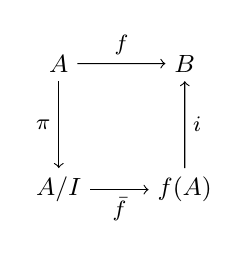
\begin{tikzpicture}[scale=1.6]
            \small
            \node (A)  at (0,1) {$A$};
            \node (AI) at (0,0) {$A/I$};
            \node (fA) at (1,0) {$f(A)$};
            \node (B)  at (1,1) {$B$};

            \footnotesize
            \draw [->] (A)  -- node[left] {$\pi$}     (AI);
            \draw [->] (AI) -- node[below]{$\bar{f}$} (fA);
            \draw [->] (fA) -- node[right]{$i$}       (B);
            \draw [->] (A)  -- node[above]{$f$}       (B);
        \end{tikzpicture}
        \caption{Noether isomorphism theorem.}
        \label{fig:NoetherIsoTrm}
    \end{figure}
    where $\bar{f}$ is an isomorphism of rings.
    \begin{proof}
        % Ignoring the second binary operation and regarding all objects as additive abelian groups, we get the above factorization where $\bar{f}$ is a bijection (additive isomorphism). This is addition to addition.
        % We also need to check multiplication to multiplication and 1 to 1.
        % $f$ is a ring homomorphism and $i$ is a one-to-one ring homomorphism. Thus, $\bar{f}\circ\pi$ is a ring homomorphism. This combined with the fact that $\pi$ is an onto ring homomorphism implies that $\bar{f}$ is a ring homomorphism (we can write this out in grueling detail for ourselves; Nori accidentally did this last class. The language here is not intended to confuse; this is intuitive -- we can add rigor ourselves).
        % We technically need the definition of an isomorphism of rings to complete our theorem.


        If we ignore $\times$ and regard $A,B$ as additive abelian groups, the FIT applies and yields the above (unique) factorization. In it, $\bar{f}$ is a bijective additive isomorphism (group homomorphism). Thus, this takes care of proving that $\bar{f}$ respects addition.\par
        We now just need to prove that $\bar{f}$ respects multiplication and sends 1 to 1 to complete our verification that it is a ring homomorphism. We will do this indirectly. First, observe that $f$ is a ring homomorphism and $i$ is a one-to-one ring homomorphism (really; do you mean that $i$ is one-to-one with the subset $f(A)\subset B$ so that defining $i^{-1}\circ f$ makes sense??). Thus, $\bar{f}\circ\pi=i^{-1}\circ f$ is a ring homomorphism (as we can confirm). This combined with the fact that $\pi$ is onto implies that $\bar{f}$ is a ring homomorphism (as we can confirm).\par
        This essentially completes our proof; we just need the formal definition of an isomorphism of rings to take it to the finish line.
    \end{proof}
    \item Notes on the Noether Isomorphism Theorem.
    \begin{itemize}
        \item Nori leaves out some of the grueling detail in this proof in favor of a simple statement of the idea (the "as we can confirm" statements) because we can work out that detail for ourselves.
        \begin{itemize}
            \item Nori accidentally presented all of the detail last class, and people got very confused.
            \item The language used in the proof we have now is not intended to confuse but to provide intuition; we can investigate rigor to whatever depth we choose.
        \end{itemize}
        \item More on the structure of the decomposition: $\pi$ is the canonical surjection and $i$ is the canonical injection; $\bar{f}$ is in the middle.
    \end{itemize}
    \item \textbf{Isomorphism} (of rings): A ring homomorphism $f:A\to B$ for which\dots
    \begin{enumerate}[label={(\roman*)}]
        \item There exists a corresponding ring homomorphism $g:B\to A$ such that\dots
        \item $f\circ g=\id_A$ and $g\circ f=\id_B$.
    \end{enumerate}
    \item Notes on the definition of an isomorphism of rings.
    \begin{itemize}
        \item If $f$ is a ring homomorphism, then (ii) implies that $f$ is a bijection of sets.
        \begin{itemize}
            \item Implication: If $f$ is a ring homomorphism and if $f$ is a bijection, then there exists a function $g:B\to A$ such that (ii) holds.
            \item It is fairly clear that this $g$ is also a ring homomorphism.
        \end{itemize}
        \item "Iso" means bijective homomorphism.
        \item We need bijective because continuous functions don't have continuous inverses??
    \end{itemize}
    \item Let's go back to talking about ideals.
    \item \textbf{Principle left ideal}: An ideal of the following form, where $R$ is a ring and $b\in R$. \emph{Denoted by} $\bm{Rb}$. \emph{Given by}
    \begin{equation*}
        Rb = \{ab\mid a\in R\}
    \end{equation*}
    \begin{itemize}
        \item $(Rb,+)$ is an additive subgroup of $R$.
        \begin{itemize}
            \item This follows from the fact that $r_b:(R,+)\to(R,+)$ is a group homomorphism and $Rb$ is equal to the image $r_b(R)$ of $R$ under this group homomorphism.
        \end{itemize}
        \item This motivates the linear algebra exercises in HW2??
        \item There also exist principal right ideals and principle two-sided ideals.
        \item It is correct that $Rb$ is a principal "left" ideal (closed under \emph{left} multiplication), even though $Hg$ is a "right" coset (multiplying the coset by an element of $G$ on the right).
    \end{itemize}
    \item Let $c\in R$, let $h\in Rb$. Is $ch\in Rb$?
    \begin{itemize}
        \item Yes, because $h=ab$ implies that there exists $a\in R$ such that $ch=(ca)b\in Rb$. Check??
    \end{itemize}
    \item We now look at three constructions originating from ideals: Sums, intersections, and products.
    \item \textbf{Sum} (of ideals): The ideal defined as follows, where $I,J\subset R$ are ideals. \emph{Denoted by} $\bm{I+J}$. \emph{Given by}
    \begin{equation*}
        I+J = \{a+b\mid a\in I,b\in J\}
    \end{equation*}
    \begin{itemize}
        \item Definitions for left, right, and two-sided ideals.
        \item We can check all of the properties to confirm that this is an ideal.
        \item Let $\alpha\in R$, $\alpha I\subset I$.  Well $\alpha I\subset J$ implies $\alpha(I+J)\subset I+J$.
    \end{itemize}
    \item Let $\{I_\lambda\}_{\lambda\in\Lambda}$ be a (finite??) family of ideals (left, right, or two-sided). Then
    \begin{equation*}
        \sum_{\lambda\in\Lambda}I_\lambda = \{a_1+a_2+\cdots+a_n\mid n\in\N,a_i\in I_{\lambda_i}\text{ for some }\lambda_i\in\Lambda\}
    \end{equation*}
    is a (left, right, or two-sided) ideal.
    \item Example: Given $a_1,a_2\in R$, $Ra_1+Ra_2$ is a left ideal.
    \begin{itemize}
        \item Note that it is not a principal ideal, however.
    \end{itemize}
    \item $R$ a ring implies that $R[X]$ is a ring, which in turn implies that $R[X][Y]=R[X,Y]$ is also a ring.
    \begin{itemize}
        \item Let $R[X,Y]=A$ and $R=\R$. Then, for instance,
        \begin{equation*}
            AX+AY = \{f(X,Y)X+g(X,Y)Y\mid f,g\in A\}
        \end{equation*}
        \item All of these functions vanish at $(0,0)$. Thus, this ideal is not principal??
        \begin{itemize}
            \item It'll be a while before we treat such rings formally.
            \item We can take this claim as an exercise for now, though (see below).
        \end{itemize}
        \item Note that similarly, $AX$ is the set of all functions vanishing on the $y$-axis.
    \end{itemize}
    \item Exercise: Prove that $AX+AY$ is not a principal ideal.
    \item \textbf{Intersection} (of ideals): The ideal defined as follows, where $\{I_\lambda\}_{\lambda\in\Lambda}$ is a family of ideals. \emph{Given by}
    \begin{equation*}
        \bigcap_{\lambda\in\Lambda}I_\lambda
    \end{equation*}
    \begin{itemize}
        \item Definitions for left, right, and two-sided ideals.
        \item Easy said aloud, not written down??
    \end{itemize}
    \item \textbf{Product} (of ideals): The ideal defined as follows, where $I,J$ are ideals. \emph{Denoted by} $\bm{IJ}$. \emph{Given by}
    \begin{equation*}
        IJ = \{a_1b_1+a_2b_2+a_nb_n\mid n\in\N,\ a_1,\dots,a_n\in I,\ b_1,\dots,b_n\in J\}
    \end{equation*}
    \begin{itemize}
        \item Note that $IJ\neq\{ab\mid a\in I,b\in I\}$. This is not even a subgroup under addition.
        \item $IJ$ as defined, however, is a subgroup with respect to $+$.
        \item The fact that $IJ$ is an ideal is justified by the distributive law:
        \begin{equation*}
            \alpha(a_1b_1)+\cdots+\alpha(a_nb_n) = (\alpha a_1)b_1+\cdots+(\alpha a_n)b_n
        \end{equation*}
        \begin{itemize}
            \item Note that the term on the far right is an element of $IJ$ since $\alpha a_i\in I_{\lambda_i}$ by the definition of $I_{\lambda_i}$ as an ideal.
        \end{itemize}
        \item Alternate form:
        \begin{equation*}
            IJ = \sum_{b\in J}Ib
        \end{equation*}
    \end{itemize}
    \item Let $R$ be a commutative ring, and let $I,J$ be ideals. Do we know that $IJ\subset I$?
    \begin{itemize}
        \item Yes, since the set is closed under multiplication as an ideal.
        \begin{itemize}
            \item In particular, $a\in I$ and $b\in R$ imply $ab\in I$.
        \end{itemize}
        \item Same logic: $IJ\cap J$.
        \item Combining these results: $IJ\subset I\cap J$.
        \item $IJ=I\cap J$ iff $I,J$ are both two-sided ideals??
        \item In fact, if $I$ is a left ideal and $J$ is a right ideal, then $IJ$ is a 2-sided ideal.
    \end{itemize}
    \item Example: Let $R=\Z$.
    \begin{itemize}
        \item Then ideals $I,J$ are necessarily of the form $I=\Z d$, $J=\Z e$ for $d,e\in R$.
        \item It follows that $IJ=\Z de$ and $I\cap J=\Z f$ where $f=\lcm(d,e)$.
    \end{itemize}
    \item We now start talking about the rings we'll focus on for the rest of the course.
    \item Zero rings.
    \begin{itemize}
        \item Nothing much to be said here.
    \end{itemize}
    \item \textbf{Field}: A commutative ring $F$ such that\dots
    \begin{enumerate}[label={(\roman*)}]
        \item $0_F\neq 1_F$.
        \item $a\in F$ and $a\neq 0$ implies that there exists $b\in F$ such that $ab=1$.
    \end{enumerate}
    \item Observation: If $I\subset F$ is an ideal in a field $F$, then either $I=\{0\}$ or $I=F$.
    \begin{proof}
        If $I\neq\{0\}$, then there exists $a\in I$ which is nonzero. It follows since $F$ is a field that $1=a^{-1}a\in I$. Therefore, $b=b\cdot 1\in I$ for all $b\in F$, i.e., $I=F$.
    \end{proof}
    \item The converse of this observation is also true (for commutative rings).
    \begin{itemize}
        \item Namely, if the only ideals of a commutative ring $R$ are $\{0\}$ and $R$, then $R$ is a field.
    \end{itemize}
    \item Examples of fields: $\Q$, $\R$, $\C$, $\Z/p\Z$ where $p$ is prime.
    \begin{itemize}
        \item $\Z\subset\Q$ is not a field.
    \end{itemize}
    \item \textbf{Integral domain}: A commutative ring $A$ for which
    \begin{enumerate}
        \item $0_A\neq 1_A$;
        \item $a,b\in A$, $a\neq 0$, and $ab=0$ imply $b=0$.
    \end{enumerate}
    \item The cancellation lemma holds in integral domains.
    \begin{itemize}
        \item Namely, if $A$ is an integral domain and $a,b,c\in A$, then $ab=ac$ and $a\neq 0$ imply that $b=c$.
    \end{itemize}
\end{itemize}



\section{Office Hours (Callum)}
\begin{itemize}
    \item HW1 Q11.
    \begin{itemize}
        \item I need to factor in some $-1$'s to account for all integers $\Z$.
    \end{itemize}
    \item Do we have to justify $0\cdot x=0$ in our proof of HW1 Q1?
    \begin{itemize}
        \item It's ok to assume things like this that were either covered in class or in the relevant sections of \textcite{bib:DummitFoote}.
    \end{itemize}
    \item Do we need to go more formal for HW1 Q2, explaining different forms of addition, functional equality, etc.?
    \item Additional sophistication in HW1 Q10?
    \item Using HW1 Q7 to solve HW1 Q9?
    \begin{itemize}
        \item Use the diagonal $\Delta:R\to R\times R$\footnote{It is standard notation to use $\Delta$ for this function.} defined by $r\mapsto(r,r)$.
        \item We know that $\Delta$ is a ring homomorphism (see HW1 Q4) and that $A\times B\subset R\times R$ is a subring.
        \item It follows from the set theoretic definition that $A\cap B=\Delta^{-1}(A\times B)$; apply HW 1 Q7.
    \end{itemize}
\end{itemize}



\section{Properties of Ideals}
\begin{itemize}
    \item \marginnote{1/13:}\textbf{Integral domain}: A commutative ring $R$ satisfying the following two conditions.
    \begin{enumerate}[label={(\alph*)}]
        \item $0_R\neq 1_R$.
        \item $a,b\in R$ with $a,b\neq 0$ implies $ab\neq 0$.
    \end{enumerate}
    \item All subrings of fields are integral domains (proved later).
    \item \textbf{Degree} (of $f\in R[X]$ nonzero): The number $\max S$, where
    \begin{equation*}
        S = \{n\in\Zg\mid a_n\neq 0\}
    \end{equation*}
    \emph{Denoted by} $\bm{\deg(f)}$.
    \begin{itemize}
        \item Some people call the degree of the zero polynomial "$-1$."
        \item $f$ a polynomial implies that $S$ is finite.
        \item $f\neq 0$ implies $S\neq\emptyset$.
    \end{itemize}
    \item \textbf{Leading coefficient} (of $f\in R[X]$ nonzero): The number $a_d$, where $d=\deg(f)$.
    \item Proposition: If $R$ is an integral domain, then $R[X]$ is an integral domain.
    \begin{proof}
        Let $f,g\in R[X]$ both be nonzero polynomials of degrees $d,e$ with leading coefficients $a_d,a_e$. In particular, let
        \begin{align*}
            f &= a_0+\cdots+a_dX^d&
            g &= b_0+\cdots+b_eX^e
        \end{align*}
        Thus, by the definition of multiplication on $R[X]$,
        \begin{equation*}
            fg = a_0b_0+\cdots+a_db_eX^{d+e}
        \end{equation*}
        Since $a_d,b_e\neq 0$ by the hypothesis that they are the leading coefficients of nonzero polynomials and since $R$ is an integral domain, we know that $a_db_e\neq 0$. Thus, $\deg(fg)=d+e$ and the leading coefficient is $a_db_e$, so $fg$ is nonzero, as desired.
    \end{proof}
    \item Corollary: $R[X][Y]=R[X,Y]$ is an integral domain.
    \item Corollary: $R[X_1,\dots,X_n]$ is an integral domain for all $n\in\N$.
    \item \textbf{Monic} (polynomial): A polynomial with leading coefficient 1.
    \begin{itemize}
        \item Examples: $1,X+a,X^2+aX+b$.
    \end{itemize}
    \item Multiplying any polynomial by a monic polynomial yields a nonzero polynomial.
    \item Exercise: If $f\in R[X]$ is monic, then $l_f:R[X]\to R[X]$ is injective.
    \begin{proof}
        Let $d=\deg(f)$ and let $e=\deg(g)$ for some nonzero $g\in R[X]$. $g\neq 0$ implies that the leading coefficient of $g$ is some $b\neq 0$. Hence, the leading coefficient of $fg$ has no term of degree greater than $d+e$, and the coefficient of the $X^{d+e}$ term is $1b$.\par
        This shows nonzero; technically also need to show distinctness under left multiplication.
    \end{proof}
    \item \textbf{Characteristic} (of a ring): The unique $d\in\Zg$ such that $\ker(j)=\Z d$, where $j:\Z\to R$ is the homomorphism defined by $m\mapsto m_R$. \emph{Denoted by} $\bm{\chr(R)}$.
    \item If $\chr(R)=1$, then $R$ is the zero ring.
    \item We have $\Z\xrightarrow{\pi}\Z/\ker(j)\hookrightarrow R$.
    \item All polynomials (the fields we have considered thus far) have characteristic 0.
    \item The subrings of an integral domain are integral domains.
    \begin{proof}
        $\chr(\text{integral domain})$ is either 0 or a prime number.
    \end{proof}
    \item Question: Given an ideal $I$ in a ring $R$, when is $R/I$ a field? An integral domain?
    \item Recall that if $R$ is a commutative ring, then TFAE.
        \begin{enumerate}
            \item $1_R\neq 0_R$ and $a\in R$, $a\neq 0$ implies that there exists $b\in R$ such that $ab=1$.
            \item There are exactly two ideals of $R$ (specifically, $\{0\}$ and $R$).
        \end{enumerate}
        \begin{proof}
            \underline{$(2)\Rightarrow(1)$} is easy. Implies $1\neq 0$ check. If $a\in R$, $a\neq 0$, then $\{0\}\subsetneq Ra$. The hypothesis implies that $Ra=R$ and $1\in R$. Thus, there exists $b\in R$ such that $ba=1$.\par
            \underline{$(1)\Rightarrow(2)$}: Not covered in class.
        \end{proof}
    \item $R$ is a field if it satisfies $1\sim 2$.
    \item Question: $I$ is an ideal of $R$. How is $\{\text{ideals in }R\}$ related to $\{\text{ideals in }R/I\}$?
    \begin{itemize}
        \item Consider the canonical surjection $\pi:R\to R/I$, often denoted by $\pi(a)=\bar{a}$ for all $a\in R$.
        \begin{enumerate}[label={(\alph*)}]
            \item If $J\subset R$ is an ideal, is $\pi(J)$ an ideal in $R/I$?
            \begin{itemize}
                \item $(J,+)$ is a subgroup of $(R,+)$. This implies that $\pi(J)$ is a subgroup of $(R/I,+)$. Let $a\in R$. Then $J$ an ideal implies that $aJ\subset J$, which implies that $\pi(a)\pi(J)=\pi(aJ)\subset\pi(J)$. If $\alpha\in R/I$, then there exists $a\in R$ such that $\pi(a)=\alpha$, so this holds, as desired.
            \end{itemize}
            \item $H\subset R/I$ is an ideal. Is $\pi^{-1}(H)$ an ideal?
            \begin{itemize}
                \item Yes.
                \item No luck required (we didn't use any assumptions). This is pretty close to a homework problem.
                \item We're assuming $I$ is a nonzero ideal here.
                \item Consider a map from the set of ideals in $R/I$ to the set of ideals of $R$ that contain $I$. $H$ is in the first set; $\pi^{-1}(H)$ is in the second set. But $\pi(\pi^{-1}(H))=H$ because $\pi$ is onto.
                \item If $H_1,H_2$ are ideals of $R/I$ and $\pi^{-1}(H_1)=\pi^{-1}(H_2)$, then $\pi\pi^{-1}H_1=\pi\pi^{-1}H_2$, i.e., $H_1=H_2$.
                \item ...
            \end{itemize}
        \end{enumerate}
    \end{itemize}
    \item Every ideal of $R/I$ equals $J/I$ for a unique ideal $J$ of $R$ such that $J\supset I$.
    \item Exercise: $R/J\cong (R/I)/(J/I)$ using nothing but the FIT.
    \item Why did we get into this discussion? Trying to figure out when a ring is a field??
    \item Let $I\subset R$ be an ideal such that $R/I$ is a field. This is true iff $R/I$ has exactly two ideals, and iff there are exactly two ideals $R\supset J\supset I$.
    \begin{itemize}
        \item This is true if $I\neq R$ and $J$ an ideal of $R$ and $I\subset J$ implies $J=R$ is called a \textbf{maximal ideal}.
        \item Ideals $I$ with this property are \textbf{maximal ideals}.
        \item Proposition: $R/I$ is a field implies $I$ is a maximal ideal.
    \end{itemize}
    \item HW3: Basic problems and some easy linear algebra problems.
    \item There will be Nori office hours on 1 day. He will come in-person unless it's very cold, and in that case, they will be virtually.
\end{itemize}



\section{Chapter 7: Introduction to Rings}
\emph{From \textcite{bib:DummitFoote}.}
\subsection*{Section 7.3: Ring Homomorphisms and Quotient Rings}
\begin{itemize}
    \item \marginnote{1/9:}Definition of a \textbf{ring homomorphism} and a \textbf{kernel} (of a ring homomorphism).
    \item \textbf{Isomorphism}: A bijective ring homomorphism. \emph{Denoted by} $\bm{\cong}$.
    \item Examples of ring homomorphisms.
    \begin{enumerate}
        \item The map $\varphi:\Z\to\Z/2\Z$ which sends even integers to 0 and odd integers to 1.
        \begin{itemize}
            \item \textcite{bib:DummitFoote} proves that this map satisfies the requisite stipulations.
            \item Note that $\varphi$ can be viewed as a projection function from the fiber bundle $\Z$ to be base space $\Z/2\Z$, where the even and odd integers are the two fibers.
        \end{itemize}
        \item $\phi_n:\Z\to\Z$ defined by $\phi_n(x)=nx$ is \emph{not} a ring homomorphism in general.
        \begin{itemize}
            \item Reason: We only have
            \begin{equation*}
                \phi_n(xy) = nxy = n^2xy = nxny = \phi_n(x)\phi_n(y)
            \end{equation*}
            when $n=n^2$, i.e., when $n=0,1$.
            \item $\phi_0$ is the \textbf{zero homomorphism} (on $\Z$) and $\phi_1$ is the \textbf{identity homomorphism} (on $\Z$).
            \item Note that $\phi_n$ is a \emph{group homomorphism} from $(\Z,+)$ to itself for all $n$.
        \end{itemize}
        \item $\varphi:\Q[X]\to\Q$ defined by $\varphi(p)=p(0)$.
        \begin{itemize}
            \item Just like the evaluation function discussed in class.
            \item $\ker\varphi$ is the set of all polynomials with constant term 0.
        \end{itemize}
    \end{enumerate}
    \item Images and kernels of ring homomorphisms are subrings.
    \begin{proposition}\label{prp:7.5}
        Let $R,S$ be rings and let $\varphi:R\to S$ be a homomorphism.
        \begin{enumerate}
            \item The image of $\varphi$ is a subring of $S$.
            \item The kernel of $\varphi$ is a subring of $R$. Furthermore, if $\alpha\in\ker\varphi$, then $r\alpha,\alpha r\in\ker\varphi$ for every $r\in R$, i.e., $\ker\varphi$ is closed under multiplication by elements from $R$.
        \end{enumerate}
        \begin{proof}
            Given.
        \end{proof}
    \end{proposition}
    \item Motivating the definition of a quotient ring.
    \begin{itemize}
        \item Let $\varphi:R\to S$ have kernel $I$.
        \item The fibers of $\varphi$ are the additive cosets $r+I$ of the kernel $I$.
        \item Recall that in the FIT, we saw that the fibers of $\varphi$ have the structure of a group naturally isomorphic to the image of $\varphi$, which led to the notion of a quotient group by a normal subgroup.
        \item An analogous result holds for rings, i.e., the fibers of a ring homomorphism have the structure of a ring naturally isomorphic to the image of $\varphi$, and this motivates the definition of a quotient ring.
        \item The whole passage about this on \textcite[240-41]{bib:DummitFoote} is very well written and worth rereading!
    \end{itemize}
    \item \textcite{bib:DummitFoote} motivates ideals from the perspective of, "what properties must $I$ have such that $R/I$ is a subring?"
    \item "The ideals of $R$ are exactly the kernels of the ring homomorphisms of $R$ (the analogue for rings of the characterization of normal subgroups as the kernels of group homomorphisms)" \parencite[241]{bib:DummitFoote}.
    \item \textcite{bib:DummitFoote} motivates and defines the definition of \textbf{ideals}.
    \begin{itemize}
        \item There are differences from the in-class definition, though: In particular, according to \textcite{bib:DummitFoote}'s definition of subrings, an ideal is a subring, but according to the in-class definition (which additionally requires that $1_R\in I$), ideals are not subrings in general.
        \item All definitions of an ideal coincide for commutative rings.
    \end{itemize}
    \item $R/I$ is a ring iff $I$ is an ideal.
    \begin{proposition}\label{prp:7.6}
        Let $R$ be a ring and let $I$ be an ideal of $R$. Then the (additive) quotient group $R/I$ is a ring under the binary operations
        \begin{align*}
            (r+I)+(s+I) &= (r+s)+I&
            (r+I)\times(s+I) &= (rs)+I
        \end{align*}
        for all $r,s\in R$. Conversely, if $I$ is any subgroup such that the above operations are well-defined, then $I$ is an ideal of $R$.
    \end{proposition}
    \item Definition of a \textbf{quotient ring}.
    \item Isomorphism theorem analogies.
    \begin{theorem}\label{trm:7.7}\leavevmode
        \begin{enumerate}
            \item (The First Isomorphism Theorem for Rings) If $\varphi:R\to S$ is a homomorphism of rings, then the kernel of $\varphi$ is an ideal of $R$, the image of $\varphi$ is a subring of $S$, and $R/\ker\varphi$ is isomorphic as a ring to $\varphi(R)$.
            \item If $I$ is any ideal of $R$, then the \textbf{natural projection} of $R$ onto $R/I$ is a surjective ring homomorphism with kernel $I$. Thus, every ideal is the kernel of a ring homomorphism and vice versa.
        \end{enumerate}
        \begin{proof}
            Given.
        \end{proof}
    \end{theorem}
    \item \textbf{Natural projection} (of $R$ onto $R/I$): The map from $R\to R/I$ defined as follows. \emph{Denoted by} $\bm{\pi}$. \emph{Given by}
    \begin{equation*}
        \pi(r) = r+I
    \end{equation*}
    \item As with groups, we shall often use the bar notation for reduction mod $I$: $\bar{r}=r+I$.
    \begin{itemize}
        \item With this notation, addition and multiplication in the quotient ring become
        \begin{align*}
            \bar{r}+\bar{s} &= \overline{r+s}&
            \bar{r}\bar{s} &= \overline{rs}
        \end{align*}
    \end{itemize}
    \item Examples.
    \begin{enumerate}
        \item $R$ and $\{0\}$ are ideals. \textbf{Trivial} and \textbf{proper} ideals.
        \item $n\Z$ for any $n\in\Z$.
        \begin{itemize}
            \item These are also the only ideals of $\Z$ since they are the only subgroups of $\Z$.
            \item The associated quotient rings are $\Z/n\Z$.
            \item Addition and multiplication on $\Z/n\Z$ is re-explained as normal addition and multiplication followed by \textbf{reducing mod $\bm{n}$}.
        \end{itemize}
        \item $I\subset\Z[X]$ consisting of all polynomials whose terms are of degree at least 2.
        \begin{itemize}
            \item Operations: Normal and then reduction, similar to Example 2.
            \item Note that $\Z[X]/I$ has zero divisors (e.g., $\bar{x}$ since $\bar{x}\bar{x}=\overline{x^2}=\bar{0}$) even though $\Z[X]$ does not.
        \end{itemize}
        \item The kernel of the \textbf{evaluation} function.
        \begin{itemize}
            \item This is the set of all functions $f:X\to A$, where $X$ is a set and $A$ is a ring, such that $f(c)=0$.
            \item Since $E_c$ is surjective (consider all constant functions), $A^X/\ker E_c\cong A$.
            \item \textcite{bib:DummitFoote} also considers the special case $C([0,1],\R)$, and notes that more generally, the fiber of $E_c$ above the real number $y_0$ is the set of all continuous functions that pass through the point $(c,y_0)$.
        \end{itemize}
        \item $\ker E_0:R[X]\to R$.
        \begin{itemize}
            \item We can compose $E_0$ with any other homomorphism from $R\to S$ to obtain a ring homomorphism from $R[X]\to S$. For instance, if the latter homomorphism is reduction mod 2, then the fibers of the overall homomorphism are the polynomials with even constant terms and those with odd constant terms.
        \end{itemize}
        \item $M_n(J)$ is a two-sided ideal of $M_n(R)$, provided $J$ is any ideal of $R$.
        \begin{itemize}
            \item This ideal is the kernel of the surjective homomorphism from $M_n(R)\to M_n(R/J)$. Example: $M_3(\Z)/M_3(2\Z)\cong M_3(\Z/2\Z)$.
            \item If $R$ is a ring with identity, then every two-sided ideal of $M_n(R)$ is of the form $M_n(J)$ for some two-sided ideal $J$ of $R$.
        \end{itemize}
        \item The \textbf{augmentation ideal}.
        \begin{itemize}
            \item The augmentation map is surjective, so the augmentation ideal is isomorphic to $R$.
            \item Another ideal in $RG$ is the formal sums whose coefficients are all equal, i.e., the $R$-multiples of $g_1+\cdots+g_n$.
        \end{itemize}
        \item $L_j\subset M_n(R)$ consisting of all $n\times n$ matrices with arbitrary entries in the $j^\text{th}$ column and zeroes in all other columns is a left ideal of $M_n(R)$.
        \begin{itemize}
            \item If $A\in L_j$ and $T\in M_n(R)$, the matrix multiplication implies that $TA\in L_j$.
            \item Showing that $L_j$ is not a right ideal: $E_{1j}\in L_j$ but $E_{1j}E_{ji}=E_{1i}\notin L_j$ if $i\neq j$.
            \item We can develop an analogous selection of right ideals in $M_n(R)$.
        \end{itemize}
    \end{enumerate}
    \item \textbf{Trivial ideal}: The ideal $\{0\}$. \emph{Denoted by} $\bm{0}$.
    \item \textbf{Proper} (ideal): An ideal $I$ such that $I\neq R$.
    \item \textbf{Reduction mod $\bm{n}$}: The natural projection $\pi:\Z\to\Z/n\Z$.
    \item \textbf{Evaluation} (at $c$): The map from $A^X\to A$, where $A$ is a ring and $X$ is a nonempty set, defined as follows, where $c\in X$. \emph{Denoted by} $\bm{E_c}$. \emph{Given by}
    \begin{equation*}
        E_c(f) = f(c)
    \end{equation*}
    \item \textbf{Augmentation map}: The map from $RG\to R$ defined as follows. \emph{Given by}
    \begin{equation*}
        \sum_{i=1}^na_ig_i \mapsto \sum_{i=1}^na_i
    \end{equation*}
    \item \textbf{Augmentation ideal}: The set of elements of $RG$ whose coefficients sum to 0.
    \begin{itemize}
        \item The kernel of the augmentation map.
        \item Example: $g_i-g_j$ is an element of the augmentation ideal for all $1\leq i,j\leq n$.
    \end{itemize}
    \item $\bm{E_{pq}}$: The matrix with 1 in the $p^\text{th}$ row and $q^\text{th}$ column and zeroes elsewhere.
    \item \marginnote{1/11:}\textcite{bib:DummitFoote} does a deep dive on reduction mod $n$ and how it relates to the foundations of \textbf{Diophantine equations} (interesting but irrelevant).
    \item The remaining isomorphism theorems.
    \begin{theorem}\label{trm:7.8}\leavevmode
        \begin{enumerate}
            \item (The Second Isomorphism Theorem for Rings) Let $A$ be a subring and let $B$ be an ideal of $R$. Then $A+B=\{a+b\mid a\in A,b\in B\}$ is a subring of $R$, $A\cap B$ is an ideal of $A$, and $(A+B)/B\cong A/(A\cap B)$.
            \item (The Third Isomorphism Theorem for Rings) Let $I,J$ be ideals of $R$ with $I\subset J$. Then $J/I$ is an ideal of $R/I$ and $(R/I)/(J/I)\cong R/J$.
            \item (The Fourth Isomorphism Theorem for Rings) Let $I$ be an ideal of $R$. The correspondence $A\leftrightarrow A/I$ is an inclusion-preserving bijection between the set of subrings $A$ of $R$ that contain $I$ and the set of subrings of $R/I$. Furthermore, $A$ (a subring containing $I$) is an ideal of $R$ if and only if $A/I$ is an ideal of $R/I$.
        \end{enumerate}
        \begin{proof}
            All proofs follow the same structure: "First use the corresponding theorem from group theory to obtain an isomorphism of \emph{additive groups} (or correspondence of groups, in the case of the Fourth Isomorphism Theorem) and then check that this group isomorphism (or correspondence, respectively) is a multiplicative map, and so defines a \emph{ring} isomorphism. In each case the verification is immediate from the definition of multiplication in quotient rings" \parencite[246]{bib:DummitFoote}.
        \end{proof}
    \end{theorem}
    \item Definition of \textbf{sum}, \textbf{product} of ideals.
    \begin{itemize}
        \item Note that $n$ is not fixed in the product definition, so that all \emph{finite} sums (not just all sums of length $n$ for $n$ fixed) are included in the set.
    \end{itemize}
    \item \textbf{$\bm{n}^\textbf{th}$ power} (of $I$): The set consisting of all finite sums of elements of the form $a_1a_2\cdots a_n$ with $a_i\in I$ for all $i$. \emph{Denoted by} $\bm{I^n}$.
    \begin{itemize}
        \item Alternate definition: Define $I^1=I$ and $I^n=II^{n-1}$.
    \end{itemize}
    \item $I+J$ is the smallest ideal of $R$ containing both $I$ and $J$.
    \item $IJ$ is an ideal contained in $I\cap J$ (but may be strictly smaller).
    \item Examples.
    \begin{enumerate}
        \item Let $I=6\Z$ and $J=10\Z$.
        \begin{itemize}
            \item $I+J$ consists of all integers of the form $6x+10y$.
            \begin{itemize}
                \item In particular, all of these integers are divisible by 2, so $I+J\subset 2\Z$. On the other hand, $2=6(2)+10(-1)\in I+J$ implies that $2\Z\subset I+J$. Therefore, $I+J=2\Z$.
                \item In general, $m\Z+n\Z=\gcd(m,n)\Z$
            \end{itemize}
            \item $IJ$ consists of all integers of the form $(6x)(10y)$ (note that this does account for all finite sums due to the distributive law), i.e., in $60\Z$.
        \end{itemize}
        \item Let $I$ be the ideal in $\Z[X]$ consisting of the polynomials with integer coefficients whose constant term is even.
        \begin{itemize}
            \item We know, for example, that $2,x\in I$. Thus, $4=2\cdot 2$ and $x^2=x\cdot x$ are elements of $I^2=II$, as is their sum $x^2+4$; however, $x^2+4$ cannot be written as a single product $p(x)q(x)$ of two elements of $I$.
        \end{itemize}
    \end{enumerate}
\end{itemize}




\end{document}